\section{Anhang}

\begin{figure}
 \centering
  \begin{subfigure}[Genauigkeit]{
 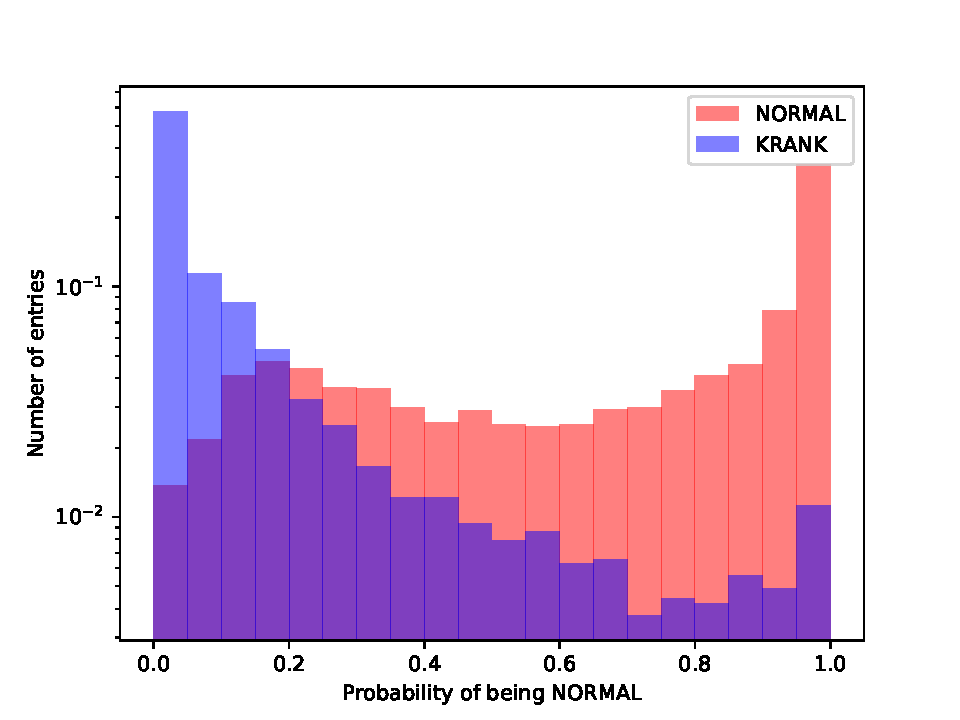
\includegraphics[width=.45\linewidth]{fig/NORMALornotlog6test.pdf}}
  \end{subfigure}
 \begin{subfigure}[Verlustfunktion]{
 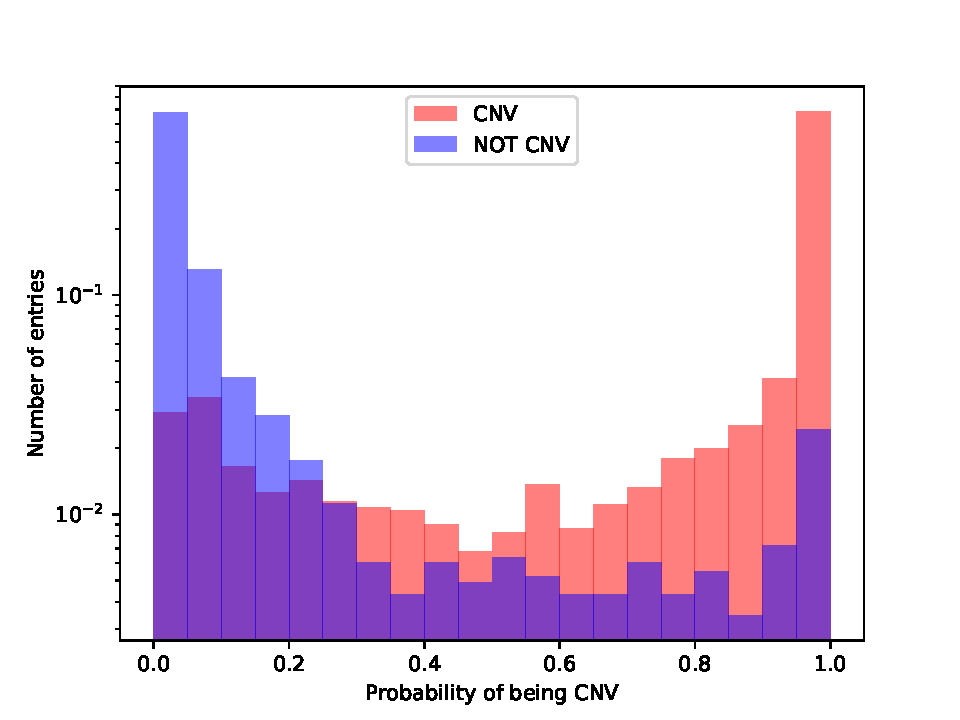
\includegraphics[width=.45\linewidth]{fig/CNVornotlog6test.pdf}}
  \end{subfigure} \\
  \begin{subfigure}[Genauigkeit]{
 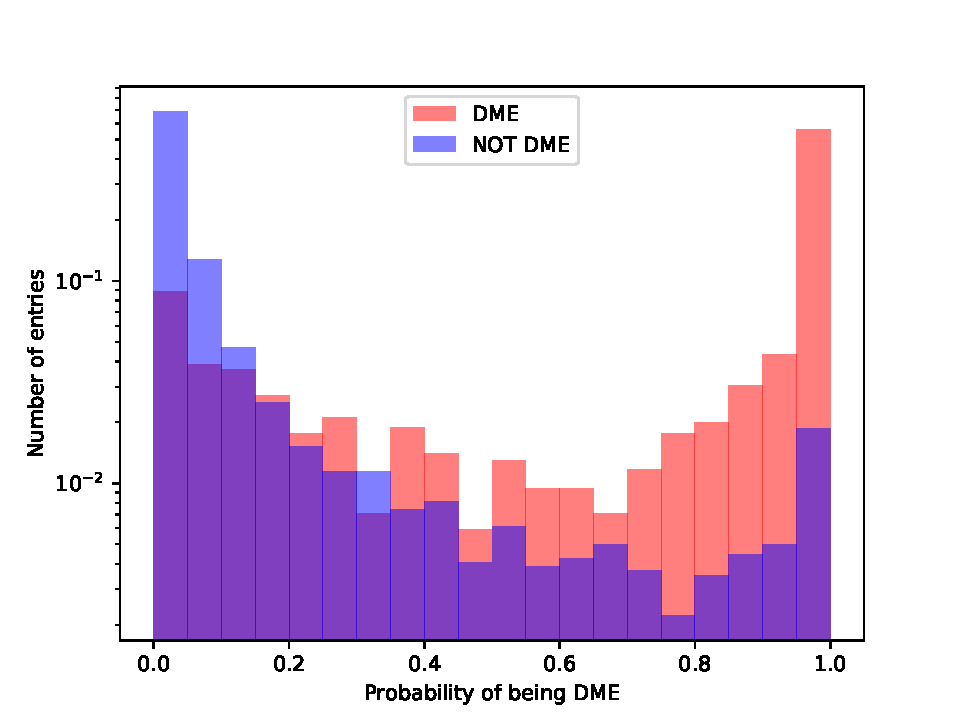
\includegraphics[width=.45\linewidth]{fig/DMEornotlog6test.pdf}}
  \end{subfigure}
 \begin{subfigure}[Verlustfunktion]{
 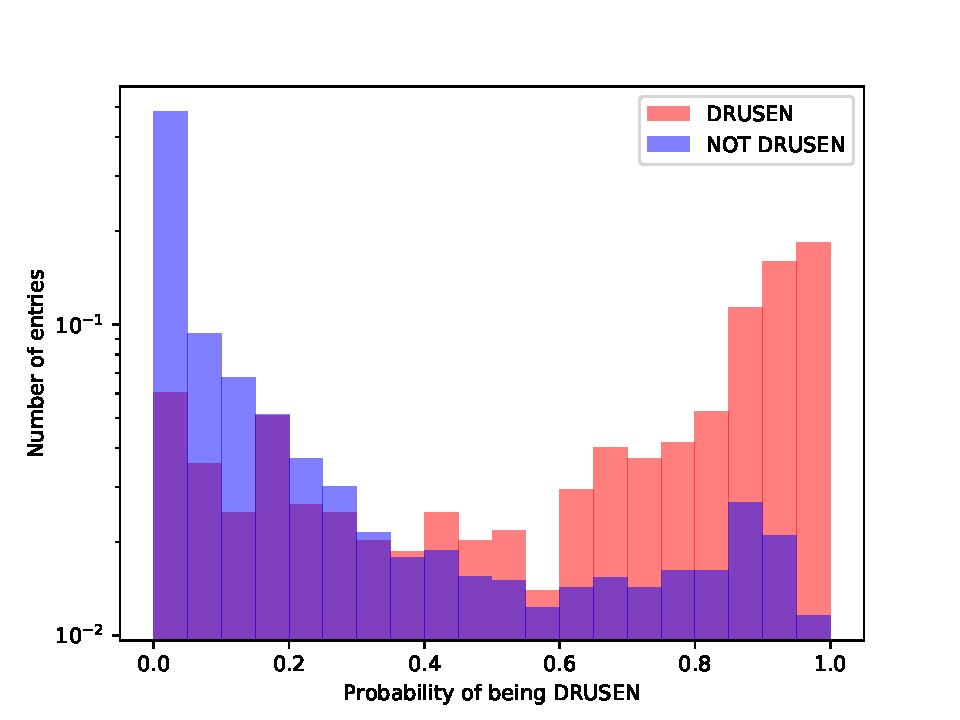
\includegraphics[width=.45\linewidth]{fig/DRUSENornotlog6test.pdf}}
  \end{subfigure}
\end{figure}


\begin{figure}[!t]
\centering
\begin{subfigure}[Normal]{
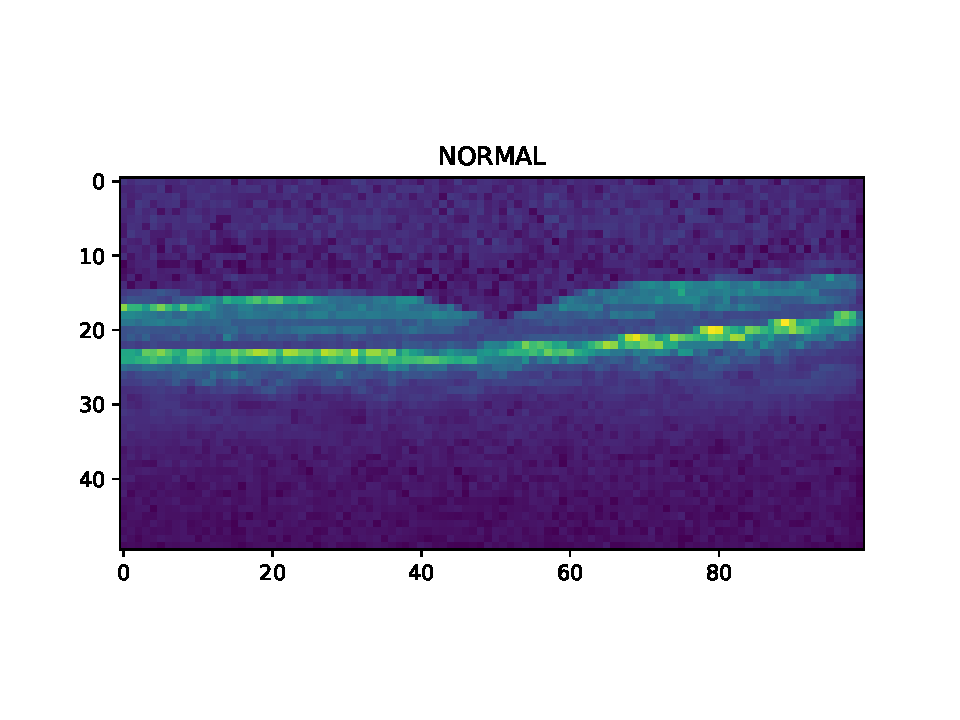
\includegraphics[width=.40\linewidth]{fig/imageNORMALscan.pdf}}
\end{subfigure}%
\begin{subfigure}[Normal]{
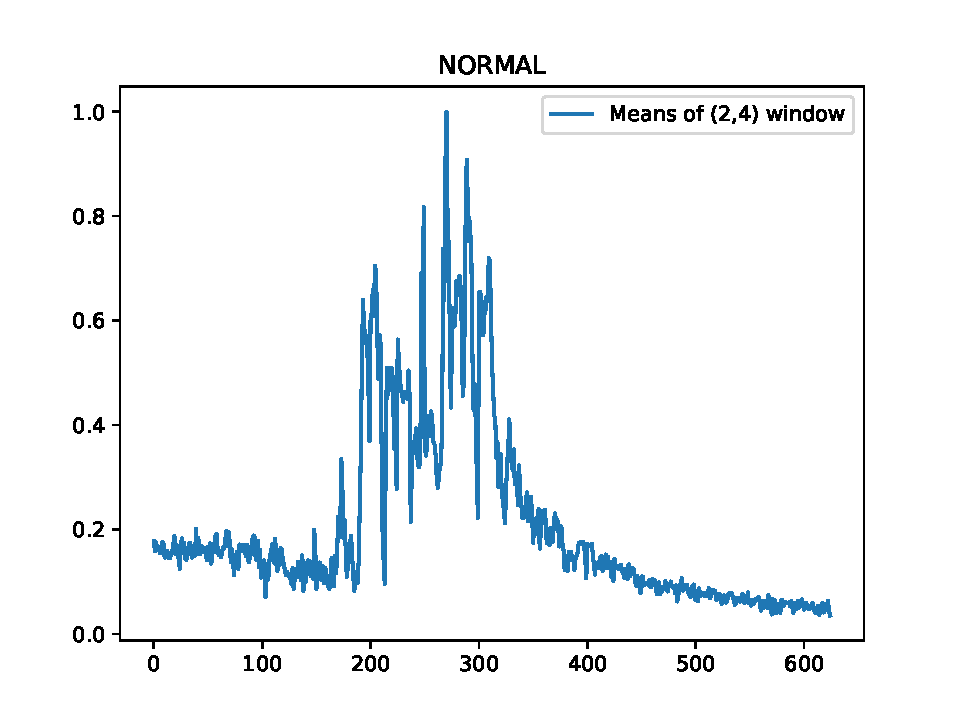
\includegraphics[width=.40\linewidth]{fig/imageNORMALmeans.pdf}}
\end{subfigure}\\
\begin{subfigure}[CNV]{
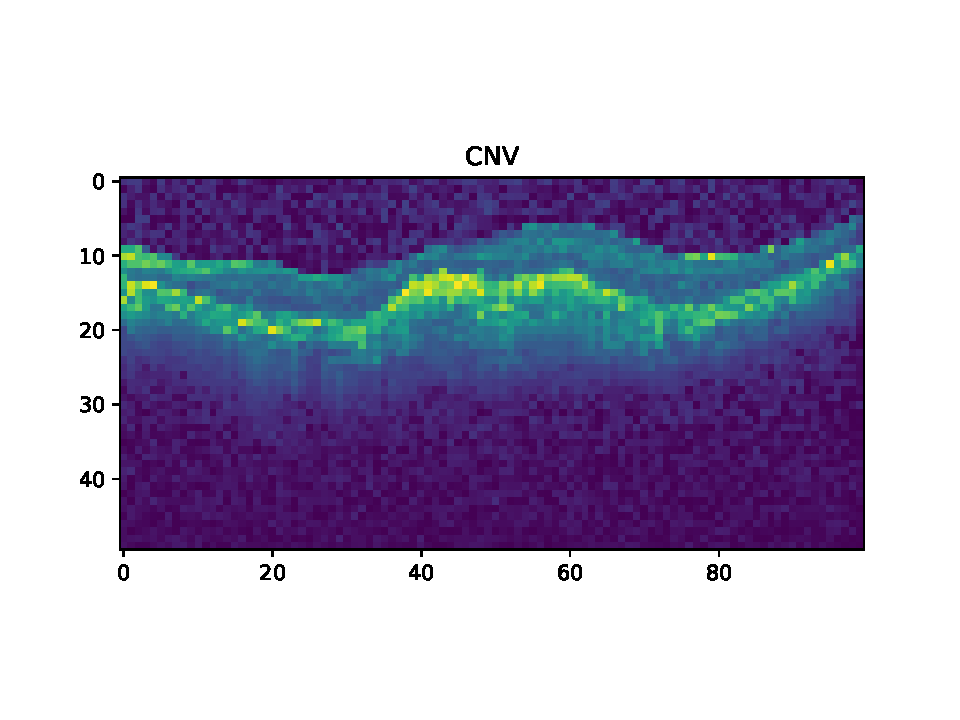
\includegraphics[width=.40\linewidth]{fig/imageCNVscan.pdf}}
\end{subfigure}%
\begin{subfigure}[CNV]{
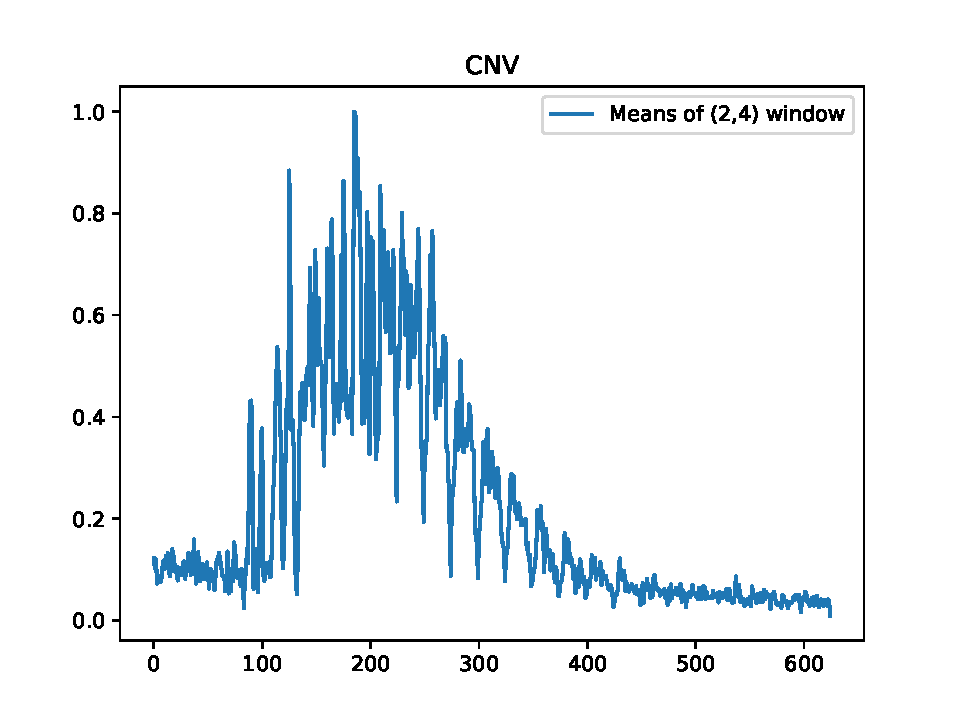
\includegraphics[width=.40\linewidth]{fig/imageCNVmeans.pdf}}
\end{subfigure}\\
\begin{subfigure}[DME]{
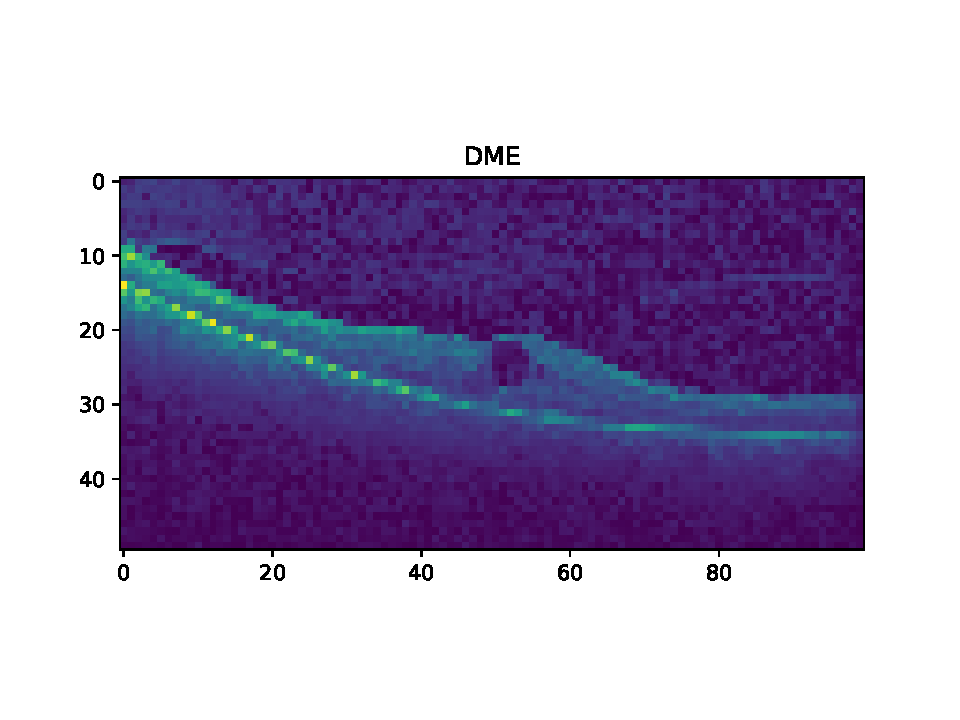
\includegraphics[width=.40\linewidth]{fig/imageDMEscan.pdf}}
\end{subfigure}%
\begin{subfigure}[DME]{
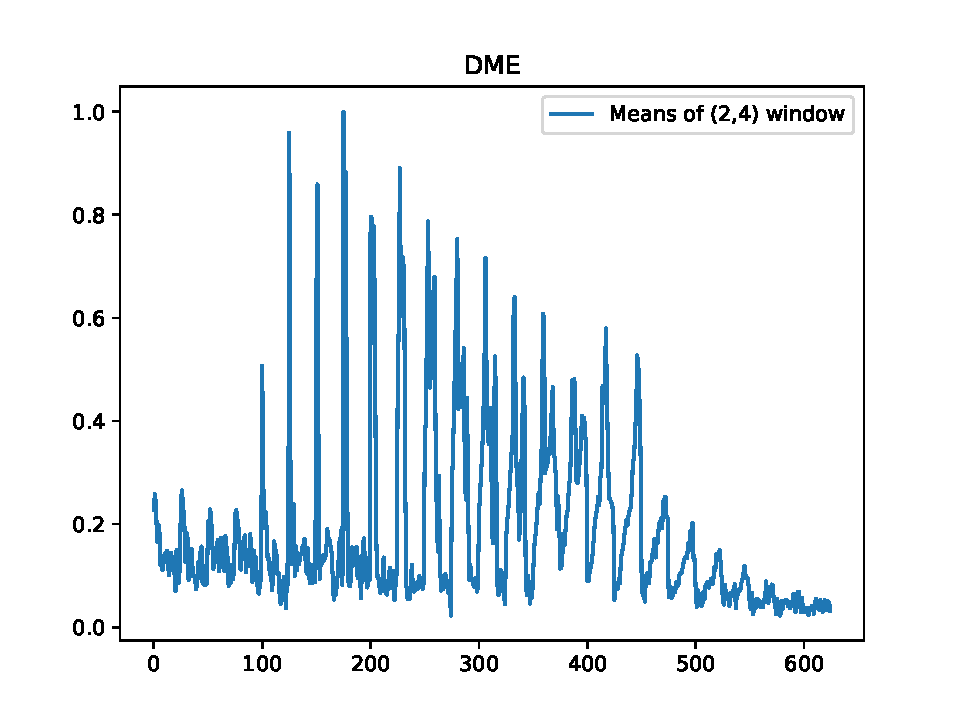
\includegraphics[width=.40\linewidth]{fig/imageDMEmeans.pdf}}
\end{subfigure}\\
\begin{subfigure}[DRUSEN]{
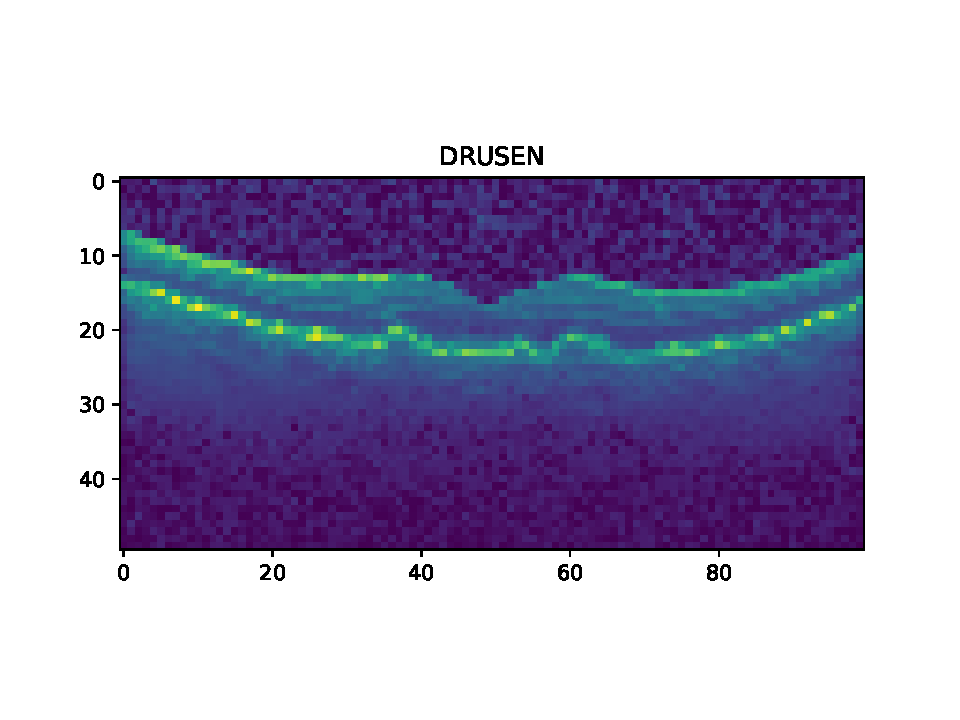
\includegraphics[width=.40\linewidth]{fig/imageDRUSENscan.pdf}}
\end{subfigure}%
\begin{subfigure}[DRUSEN]{
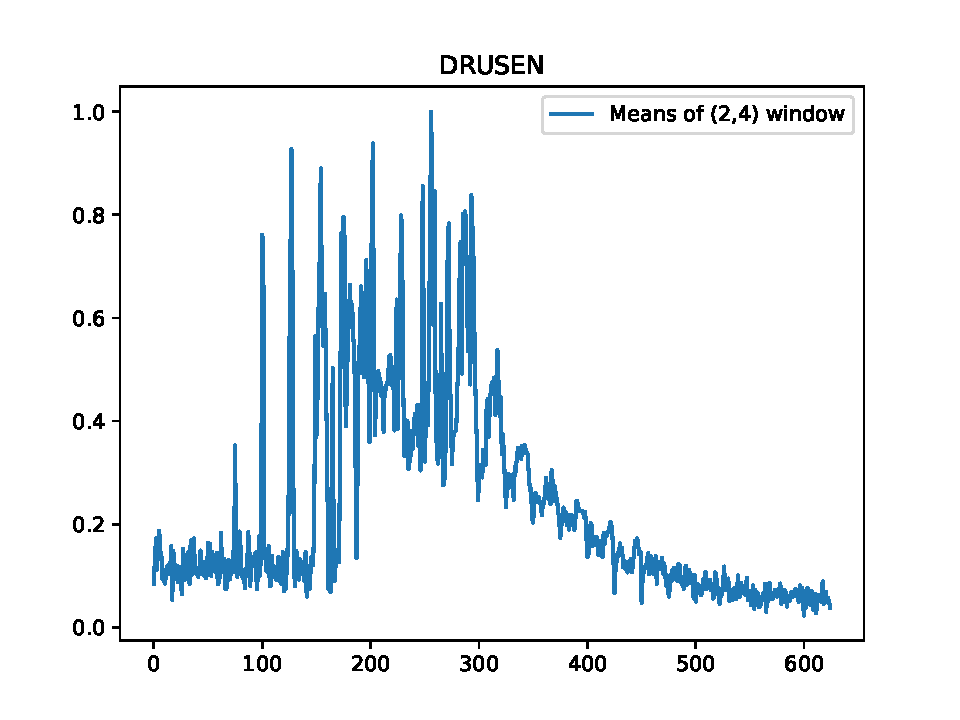
\includegraphics[width=.40\linewidth]{fig/imageDRUSENmeans.pdf}}
\end{subfigure}\\
\caption{Beispielbilder für jede der Klassen im $(50,\,100)$ Format, sowie die aus der Abrasterung durch $(2,\,4)$ Fenster erhaltene Verteilung der Mittelwerte.}
\label{fig:input}
\end{figure}%